\chapter{Previous research}
\label{chapters:previous-research}

This short chapter introduces the core concepts of the previous research that was carried out by the \textit{XML and Web Engineering Research Group} (XRG) at the Faculty of Mathematics and Physics of the Charles University in the years 2012 to 2015. Those concepts will be used for further analysis in the following chapters.

\bigskip

In 2012 XRG formalized a novel approach\footnote{The work builds on previous work of the same authors where they introduced the XSEM model \cite{necasky2007xsem}, which has later been a subject of their study.} to modeling XML schemas \cite{necasky2012conceptual} for a particular domain ontology by integrating Model Driven Development \cite{kent2002model} (specifically Model Driven Architecture) techniques to separate a conceptual mo\-del describing the domain ontology and a structural model which described the concrete XML schema.

\paragraph{Model-Driven Architecture} MDD is a software engineering technique that abstracts software development into several levels (models) to allow flexibility by separating business domain from platform decisions. MDA \cite{mda,mda_developing_in} introduced by Object Management Group (OMG) is a specialization of MDD focusing on the automation of the development of software systems.

MDA introduces four models. The topmost level CIM (Computation Independent Model) expresses the business logic and has no formal representation, as it is only a concept, hence the name computation independent. PIM (Platform Independent Model) as a second level models the business logic in UML. It does not specify a concrete platform or technology, but only the concepts in a formalized way. PSM (Platform Specific Model) reflects the formalized concepts from PIM in a platform-specific environment, such as in XML Schema, C\# or Java code, or a database schema.

The key concept is a transformation as the process of mapping the upper layer to the lower one. The transformation from CIM to PIM must be done by hand as CIM does not formally exist. More interesting is PIM to PSM transformation, as it can be automated. The transformation keeps the mapping to preserve the semantics between the models. The last level is Implementation Specific and only represents different implementations of PSM.

\bigskip

XRG used PIM and PSM in their architecture. PIM represented the domain ontology in UML-like notation\footnote{Formal definition of PIM and PSM levels is in chapter \ref{chapters:formal-background}.}, as it is independent of the platform as XML. PSM\footnote{Compared to the definition above, XRG's PSM is more like the mapping between the PIM and PSM from the MDA. Final XML Schema would then corresponds to PSM.} then represented the given schema in their own designed grammar, which was translated into a final schema, such as XSD.

\begin{figure}[h]\centering
    \begin{tikzpicture}[
        squarednode/.style={rectangle, draw=blue!60, fill=blue!5, very thick, minimum size=5mm},
    ]
        %Nodes
        \node[squarednode] (pim) at (0,0) {PIM schema};
        \node[squarednode] (psm1) at (-2.5,-1.5) {PSM schema 1};
        \node (psmDot) at (0,-1.5) {...};
        \node[squarednode] (psmN) at (2.5,-1.5) {PSM schema N};

        \node[squarednode] (schema1) at (-2.5,-3) {XML schema 1};
        \node (psmDot) at (0,-3) {...};
        \node[squarednode] (schemaN) at (2.5,-3) {XML schema N};

        \node[squarednode,cascaded] (q1) at (-1.5,-4.5) {XML queries};
        \node (psmDot) at (1,-4.5) {...};
        \node[squarednode,cascaded] (qN) at (3.5,-4.5) {XML queries};

        \node[squarednode,cascaded] (document1) at (-2.5,-6) {XML documents};
        \node (psmDot) at (0,-6) {...};
        \node[squarednode,cascaded] (documentN) at (2.5,-6) {XML documents};

        \node (psm_t)[text width=4cm,align=right] at (-7,0) {{Platform-specific level:}};
        \node (pim_t)[text width=4cm,align=right] at (-7,-1.5) {{Platform-independent level:}};
        \node (schema_t)[text width=4cm,align=right] at (-7,-3) {{Schema/Logical level:}};
        \node (ext_t)[text width=4cm,align=right] at (-7,-4.5) {{Operational level:}};
        \node (ext_t)[text width=4cm,align=right] at (-7,-6) {{Extensional level:}};

        %Lines
        \draw[-latex] (psm1) -- (pim);
        \draw[-latex] (psmN) -- (pim);
        \begin{scope}[transform canvas={xshift=-2em}]
            \draw[-latex] (document1) -- (schema1); % node[fill=white]{conforms}
            \draw[-latex] (documentN) -- (schemaN); % node[fill=white]{conforms}
        \end{scope}
        \draw[-latex] (schema1) -- (psm1);
        \draw[-latex] (schemaN) -- (psmN);
        \draw[-latex] (q1) -- (schema1);
        \draw[-latex] (qN) -- (schemaN);

        % separators
        \foreach \x in {0,...,3}{
            \draw [dotted] (-9,-0.75-1.5*\x) -- (5,-0.75-1.5*\x);
        }
    \end{tikzpicture}
    \caption{The five-level framework proposed by XRG in \cite{necasky2012conceptual}. A shared PIM layer with a conceptual model is used by multiple PSMs, where schemas are defined in their own grammar. The grammar is then translated into schemas that conform to XML documents in the last level.}
\end{figure}

The major benefit of the strategy presented is a shared conceptual model between various XML schemas, as other works at that time had a conceptual model for every schema. This was not practical as usually multiple schemas are applied in a single software. Authors have also formalized the model and have proven that their approach is correct. That means that (i) every conceptual schema models XML schema, (ii) their translation algorithm from the internal model to schema respects introduced rules and is reversible, and (iii) their normalization and optimization algorithms produce semantically same schema.

\begin{figure}[h!]
    \centering
    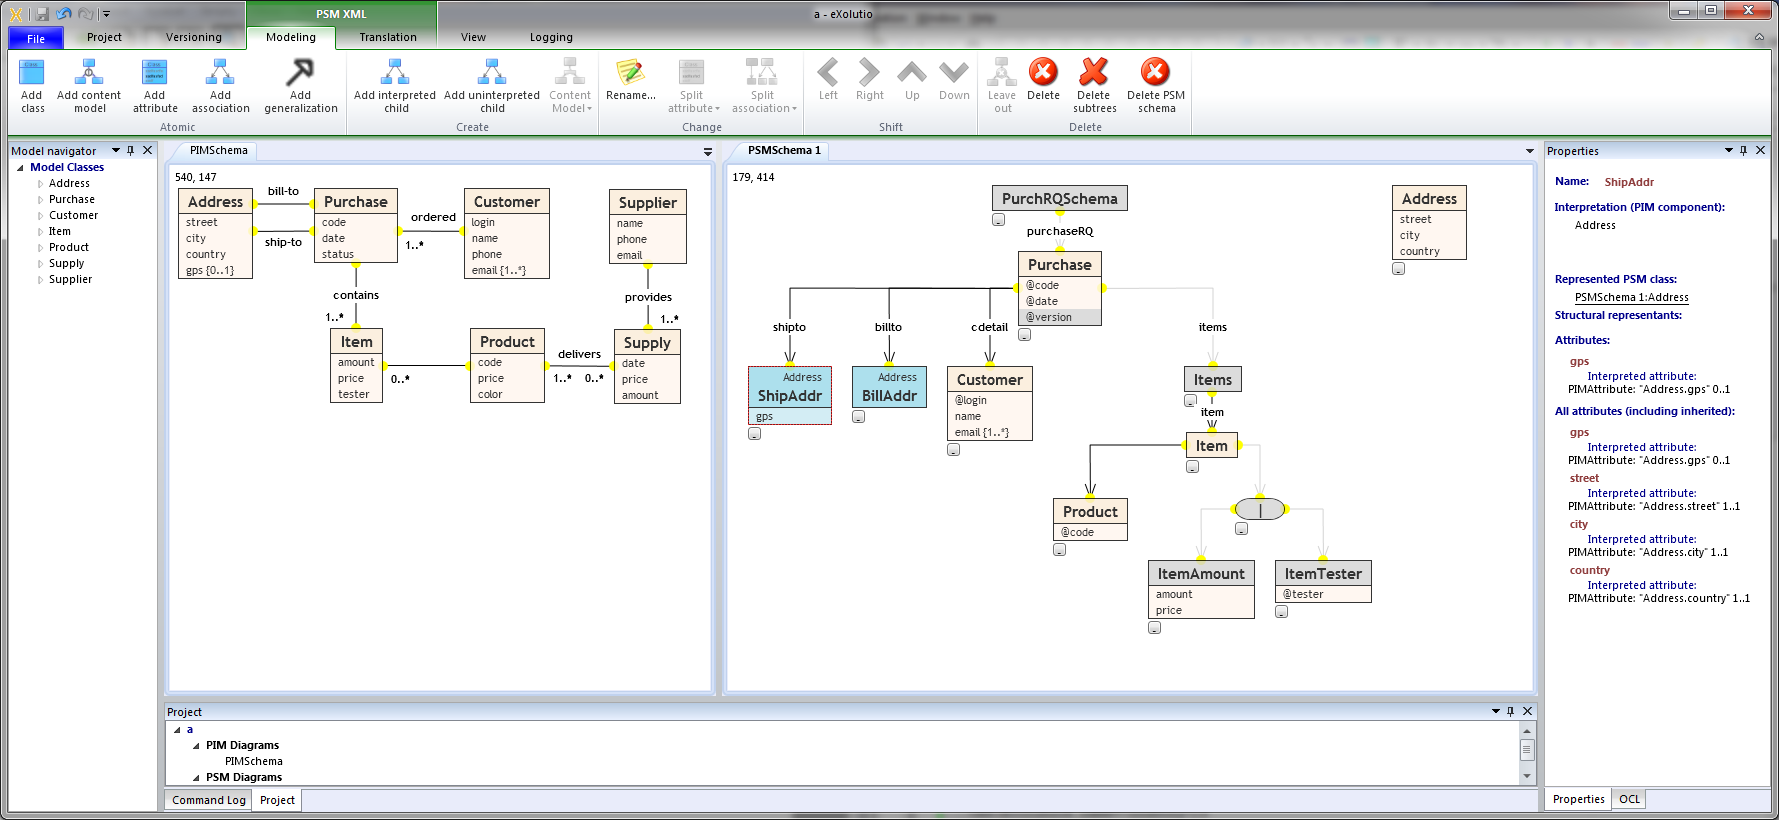
\includegraphics[width=\textwidth]{img/exolutio.png}
    \caption{Preview of the eXolutio tool. The left panel shows the PIM model as a UML class diagram, while the right panel represents a PSM schema in a tree-like structure that can be converted to an XML schema.}
    \label{fig:exolutio}
\end{figure}

Their primary use case was to create schemas for the government, such as the information system for National Register for Public Procurement (NRPP) for publishing public contracts.

\paragraph{Modeling} To create a schema, a user has to first create an ontology of desired entities as PIM. Then, multiple schemas can be created as PSM trees by first selecting a schema root and then adding entities to it. The resulting XML schemas then can be exported from the application.

\paragraph{Evolution of schemas} The focus of XRG was also directed to the evolution \cite{nevcasky2012evolution} of their proposed model to minimize the work of the data designer. As already stated in the introduction of the thesis, changes may be inevitable (either from the user requirements or from the surrounding environment) in large and complex systems, and propagating even a tiny change from the domain ontology to all affected schemas is time-consuming and error-prone.

They proposed, formalized, and later implemented a solution in restricting the changes in PIM and PSM models to only atomic operations - simple changes in the model, such as \textit{creating a new class}, \textit{updating a name of association} or \textit{removing an attribute}. Those operations are not intended to be used by the user directly but are simple enough to be formally defined and mapped to the corresponding operations in the level below. The proposed mapping is then used to propagate changes in the model to the schema level, more precisely from PSM to PIM, which is then translated to the schema level. They implemented only top-down propagation of changes as the propagation from XML documents is usually not meaningful (but theoretically possible).

\paragraph{Implementation} Their result were implemented in two tools \textit{XCase} \cite{xcase} and \textit{eXolutio} \cite{exolutio}. The former one was simpler, focused only on modeling. The latter then supported schema evolution as described in the previous section. Tools let users define the ontology from which the schemas and operations were derived for XML documents.

\paragraph{Analysis} The tool was designed only for XML, hence is not usable for other languages, such as JSON, which is very popular at the time of writing this thesis as being used by many server-centered applications to communicate with the server through the REST API \cite{fielding2000architectural}, for no-SQL databases\footnote{\url{https://www.mongodb.com/}}\footnote{\url{https://rethinkdb.com/}} and more. Nevertheless, we can use their findings and generalize the model for other formats.

They focused on the correctness and completeness of the model, which in some cases may be a limitation, such as more complex implementation and processing of the model to not allow a user to create a schema that is not valid.

Lastly, the tools didn't support sharing and collaboration, as at that time this was not considered standard practice in the industry.